\chapter{Grundlagen}
\section{Laserlichtschneiden}

Beim Laserlichtschneiden wird ein fokussierter Laserstrahl auf die Werkstückoberfläche gerichtet. Das Material schmilzt lokal auf und wird mit einem zugeführten Gas aus dem Schnittspalt ausgeblasen. So entsteht eine schmale, definierte Trennfuge. Die grundlegenden Begriffe und Kenngrößen (z.\,B.\ Strahlleistung, Strahlqualität, Fokuslage) sind in \parencite{ISO11145-2018} beschrieben.

In der Produktion kommen vor allem Faser- und Scheibenlaser zum Einsatz. CO\textsubscript{2}-Laser werden seltener verwendet. Faser- und Scheibenlaser erlauben hohe Energiedichten im Brennfleck und damit hohe Schnittgeschwindigkeiten, besonders bei dünnen bis mittleren Blechdicken. Die Wahl des Prozessgases beeinflusst Schnittqualität und Kantenfarbe. Beim Schneiden mit Stickstoff bildet sich kaum Oxid an der Schnittkante, die Kante bleibt hell und metallisch. Das ist vorteilhaft, weil in der Regel weniger Nacharbeit erforderlich ist, wie z.B dem Nachbürsten der Kante, so dass wieder eine metalische Oberfläche zu sehen ist. Beim Schneiden mit Sauerstoff reagiert das Material mit dem Gas und somit entsteht eine dunkle Oxidschicht, die die Kante verfärbt. Der Prozess kann zwar schneller sein, führt aber demanch zu zusätzlicher Nacharbeit, wenn eine helle und einwandfreie Kante gefordert ist.

Die wichtigsten Einstellgrößen dieser sind die Laserleistung, Schnittgeschwindigkeit, Fokuslage und Gasdruck. Eine höhere Leistung erlaubt höhere Geschwindigkeit, bis die Qualitätsgrenzen erreicht sind. Eine unpassende Fokuslage führt schnell zu Grat oder unvollständigem Materialaustrag. Der Gasdruck muss so gewählt werden, dass die Schmelze zuverlässig aus dem Schnittspalt entfernt wird, ohne die Kante aufzurauen. Für die Bewertung der Schnittqualität sind u.\,a.\ Grat und Rauheit relevant. ISO~9013 fasst hierfür Klassen und Toleranzen zusammen \parencite{ISO9013-2017}.

Für Edelstahl gelten gegenüber Baustahl angepasste Einstellungen. Gründe sind unter anderem eine höhere Reflexion und eine geringere Wärmeabfuhr. In der Praxis bedeutet das, dass die Leistung und die Fokuslage sorgfältig abgestimmt werden müssen. Die Geschwindigkeit muss demnach passend gewählt werden. Als Prozessgas wird meistens Stickstoff eingesetzt, um eine helle Kante und geringen Grat zu erreichen.

\section{Grat und Rauheit eines Blechteils}
\label{sec:grat-rauheit}

Grat und Rauheit beschreiben die Qualität der Schnittkante. Der Grat ist ein aufgeworfener Materialrand an der Unterkante. Er entsteht durch unvollständigen Schmelzaustrag oder durch Anhaften von Schmelze im Schnittspalt. Die Rauheit beschreibt die feinen Höhenabweichungen der Schnittfläche entlang eines Profils \(Z(x)\).

Die in Tabelle~\ref{tab:symbole-rauheit-grat} zusammengefassten Formelzeichen werden in diesem Dokument verwendet.
\begin{table}[htbp]
  \centering
  \ra{1.2}
  \caption{Formelzeichen für Rauheit und Grat}
  \label{tab:symbole-rauheit-grat}
  \begin{tabular}{@{}lll@{}}
    \toprule
    Zeichen & Bedeutung & Typische Einheit \\
    \midrule
    $Z(x)$      & gefiltertes Profil entlang der Auswertelänge $L$ & $\mu$m \\
    $Z_i$       & diskreter Profilwert an Position $x_i$            & $\mu$m \\
    $L$         & Auswertelänge                                      & mm \\
    $n$         & Anzahl der Stützstellen in $L$                     & -- \\
    $X_{s,j}$   & $j$-te Teilstrecke innerhalb von $L$               & mm \\
    $R_a$       & arithmetischer Mittenrauwert                       & $\mu$m \\
    $R_z$       & mittlere Rautiefe aus fünf Teilstrecken            & $\mu$m \\
    $P^{\max}_{j}$, $P^{\min}_{j}$ & höchster bzw.\ tiefster Punkt in $X_{s,j}$ & $\mu$m \\
    $h_b$       & Grathöhe an der unteren Schnittkante               & $\mu$m \\
    \bottomrule
  \end{tabular}
\end{table}

Die Berechnung der Kenngrößen folgt den veröffentlichten Rechenregeln. Der arithmetische Mittenrauwert \(R_a\) ist das Mittel der Beträge der Profilabweichung über die Auswertelänge \(L\) \parencite{MitutoyoQuickGuide}:
\[
R_a=\frac{1}{L}\int_{0}^{L}\lvert Z(x)\rvert\,\mathrm{d}x
\]
und in diskreter Form mit \(n\) Stützstellen \(Z_i\):
\[
R_a=\frac{1}{n}\sum_{i=1}^{n}\lvert Z_i\rvert.
\]
Die mittlere Rautiefe \(R_z\) wird über fünf Teilstrecken \(X_{s,1}\) bis \(X_{s,5}\) bestimmt \parencite{KeyenceISO4287}. In jeder Teilstrecke wird die Differenz zwischen höchstem und tiefstem Profilpunkt gebildet. \(R_z\) ist das arithmetische Mittel dieser fünf Differenzen:
\[
R_z=\frac{1}{5}\sum_{j=1}^{5}\bigl(P^{\max}_{j}-P^{\min}_{j}\bigr).
\]

Die Grathöhe \(h_b\) wird als maximale positive Auslenkung des Profils im Randbereich der unteren Schnittkante bestimmt. Grundlage ist dasselbe Profil \(Z(x)\) oder ein aus einer Punktwolke abgeleitetes Profil senkrecht zur Kante. Neben \(h_b\) können Breite und Form des Grates angegeben werden.

Die Profilwerte \(Z_i\) stammen aus einer 3D-Punktwolke oder aus einer bildbasierten Profilerfassung. Aus diesen Werten werden \(R_a\) und \(R_z\) berechnet. Die Grathöhe \(h_b\) wird im Kantenbereich aus demselben Profil ermittelt.

In Abbildung~\ref{fig:roughness-profile} ist das Prinzip der Rauheitsbestimmung schematisch dargestellt. Die rote Linie markiert den Wert von \(R_a\). \(Z_i\) sind die diskreten Profilwerte. \(X_{s,j}\) kennzeichnet die Teilstrecken für die Berechnung von \(R_z\).

\begin{figure}[htbp]
  \centering
  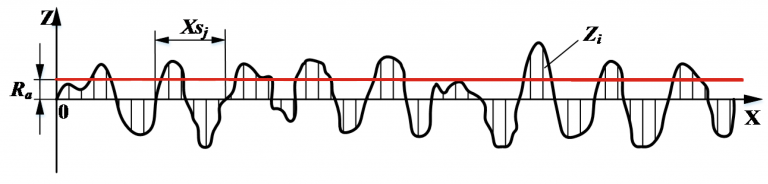
\includegraphics[width=\linewidth]{burr_roughness_schaubild.png}
  \caption[Schema zur Bestimmung der Rauheit]{Schema zur Bestimmung der Rauheit mit Profilwerten \(Z_i\), Teilstrecken \(X_{s,j}\) und markiertem \(R_a\).}
  \label{fig:roughness-profile}
\end{figure}



\section{CNNs}
-was ist

-aufbau/faltung

-anwendung